\section{Evaluation}
\label{idea-sec-evaluation}

To evaluate IDEA, we built and tested the energy-aware component and
application described in Section~\ref{idea-sec-casestudies}. For the routing
protocol, we compare our IDEA-based implementation to an approach that is not
energy-aware. For the application, we use IDEA to implement several energy
objective functions and compare their performance against each other and
against a heuristic that does not consider energy availability.

\subsection{Experimental Setup}
\label{idea-subsec-experimentalsetup}

Throughout the evaluation we present results run in several different
environments. We have implemented IDEA for TinyOS in order to run experiments
on MoteLab~\cite{motelab}, our 180~node wireless sensor network testbed. We
also present results obtained using TOSSIM~\cite{tossim}, the TinyOS
simulator. TOSSIM incorporates a closest-fit pattern matching noise model to
accurately capture complex link dynamics~\cite{cpm-ipsn07}. TOSSIM allows us
to run longer experiments incorporating various solar charging models. To
improve the realism of TOSSIM we began with a modified version developed for
the Koala project~\cite{koala-ipsn08} and performed further modifications to
correctly simulate the operation of low-power listening
(LPL), which is important to properly model the power
consumption of the radio for the ICTP experiments. We use information
collected on MoteLab to build a realistic TOSSIM radio model for our
simulations. Finally, for the application we built a Python simulator to
allow rapid prototyping of various energy objective functions.

IDEA is designed to tune components in the face of variations in both load
and charging rates, and to test this we present experiments using solar
charging data collected off of a solar panel deployed on an Arlington, MA
rooftop in March, 2009. Battery levels are calculated using a charging model
based on a Nickel-Metal Hydride battery technology with a 66\% charging
efficiency. We attenuate this data to simulate the charging produced by solar
panels of several different sizes in order to evaluate IDEA's performance as
available energy changes. We also perform experiments with a randomly
attenuated charging profile to simulate bad solar panel placement or
obstacles to incident sunlight effecting the spatial distribution of
collected energy.

For our MoteLab experiments we determine the system's ability to span periods
without charging inputs. We use two sets of initial conditions based on the
interaction between the charging data we collected and the capacity of the
batteries deployed. If the solar panel is large enough it will provide
considerable charging input and completely charge small batteries during the
day, so that all nodes begin the night with full batteries. If the solar
panel is not large enough to completely charge the batteries nodes will begin
the night with varying amounts of charge depending on their load rates during
the day.

Energy tracking is done by IDEA using a software-only approach developed for
the Pixie~\cite{pixie-sensys08} project. The component captures state
transitions and applies an energy consumption model for each state based on
current consumption measured offline. In the future we would like to
integrate a more accurate hardware-driven approach such as
iCount~\cite{icount-spots08}. The short lifetimes for some experiments are
explained by the use of extremely small batteries, which were chosen to allow
experiments to complete in reasonable amounts of time. We expect that
application developers will want to use a battery size and charging
technology suitable to allow their system to achieve a desired level of
performance, and the improvements in energy efficiency possible using IDEA
will allow smaller batteries or solar panels to be used, reducing the size
and cost of the hardware package.

Experiments for the energy-aware routing case use the first-node death energy
objective function described in
Section~\ref{idea-subsec-energyobjectivefunctions}, and therefore we evaluate
the network lifetime as the time at which the first node runs out of energy.
Our distributed localization application illustrates the process of designing
an effective energy objective function when the overall goal of the system is
known.

\subsection{ICTP: Energy-Aware Routing}

\begin{figure}[t]
\begin{center}
\textbf{(a)}\\
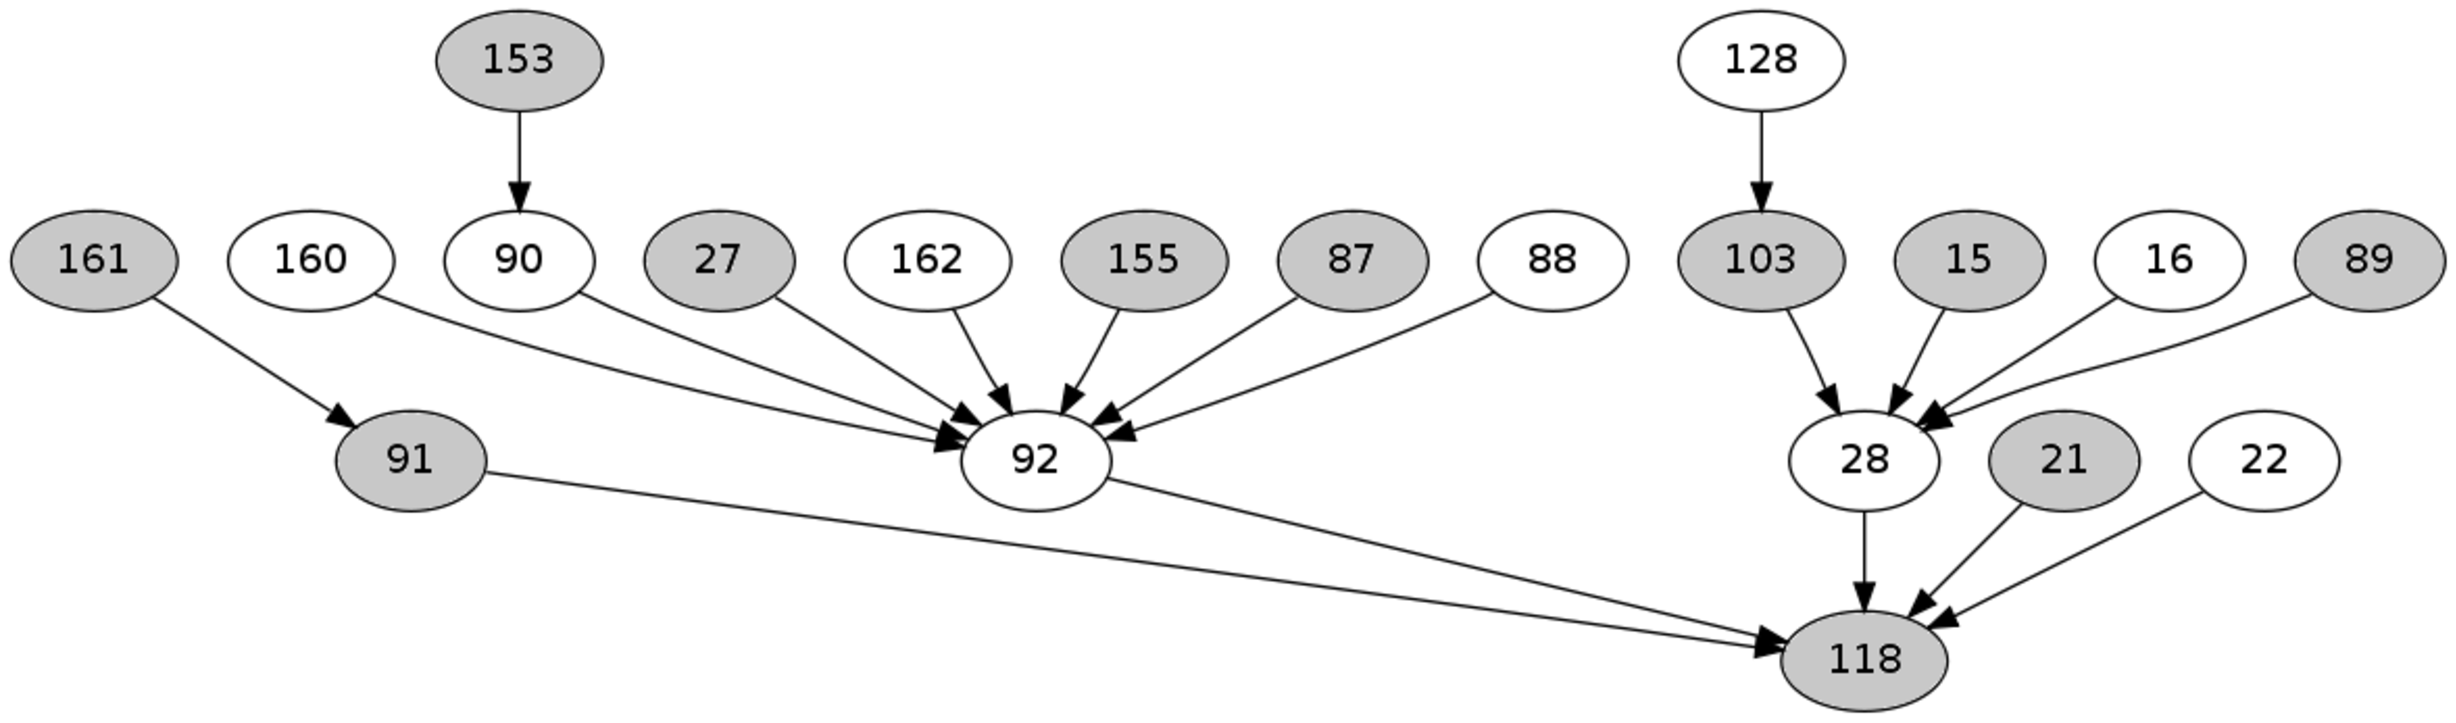
\includegraphics[width=0.7\hsize]{./5-idea/figs/ctp.pdf}\\
\textbf{(b)}\\
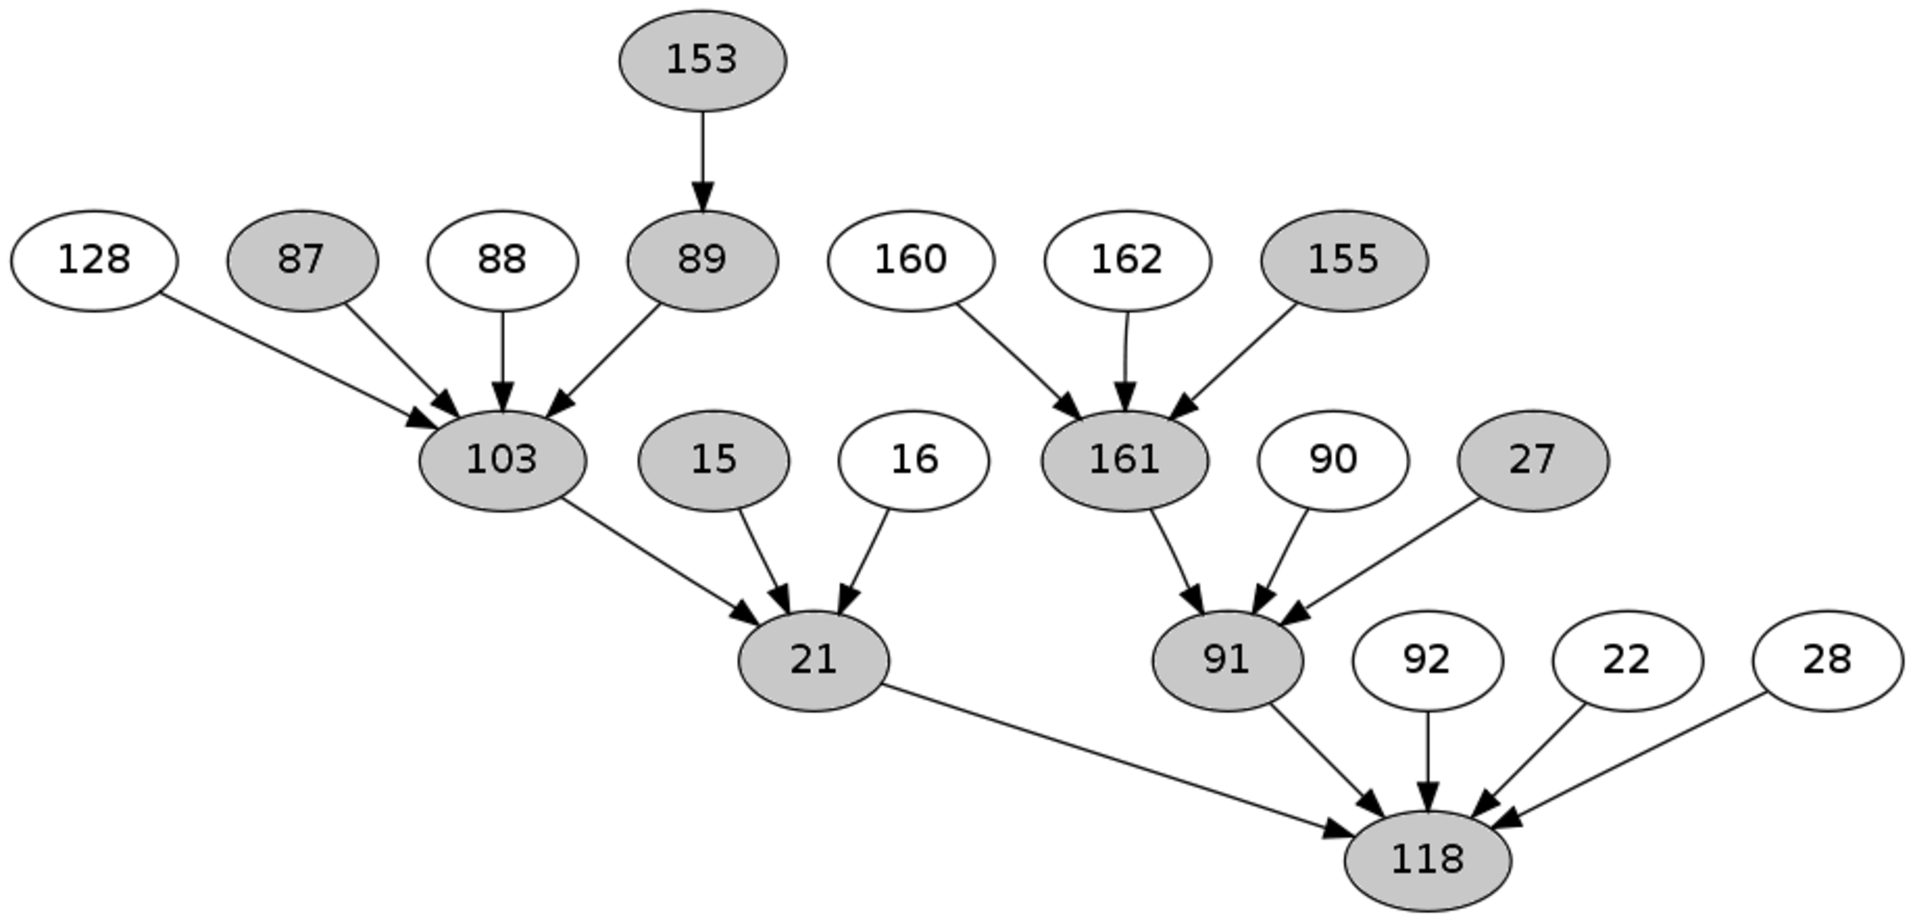
\includegraphics[width=0.7\hsize]{./5-idea/figs/ictp.pdf}\\
\end{center}

\caption{\textbf{Qualitative comparison of stock CTP and ICTP.} For this
experiment odd-numbered nodes (shaded) were set to charging rapidly, while
even-numbered nodes were not charging. Unmodified CTP builds the tree shown
in (a), which routes many packets through the even nodes. ICTP builds the
tree shown in (b), which moves all even nodes to leaf roles.}

\label{idea-fig-ictpqualitative}
\end{figure}

Using IDEA we were able to integrate energy awareness into CTP, the routing
protocol included as part of TinyOS. For these experiments each node in a
20~node network sends 6 packets to the sink per second. Static LPL intervals
of 0.5 second were used. 

Figure~\ref{idea-fig-ictpqualitative} shows a qualitative demonstration of
the difference between energy-aware and non-energy-aware routing trees. This
TOSSIM simulation ran with all odd numbered nodes charging rapidly and all
even numbered nodes not charging (with the exception of the powered sink,
Node 118). While this is an unrealistic charging pattern, it produces a clear
difference in routing protocol behavior.
Figure~\ref{idea-fig-ictpqualitative}(a) shows that unmodified CTP is unaware
of these charging differences and puts several even nodes, such as Node 92,
into positions where they are routing for multiple nodes. The total number of
nodes upstream from even numbered nodes in the stock CTP case is 14. In
contrast, ICTP realizes that the odd-numbered nodes have energy to spare and
the even-numbered nodes are lacking, and moves all even nodes to leaf roles.
None of the even nodes in Figure~\ref{idea-fig-ictpqualitative} are routing
data.

Using a 20~node subset of our MoteLab topology, we compared the performance
of ICTP to unmodified CTP using 24-hour TOSSIM simulations and the three
different solar charging scenarios previously described. As
Table~\ref{idea-table-ictpvoptimaltossim} shows, ICTP shows improvements in
lifetime over stock CTP of between 11 and 27\%. The different routing trees
formed by ICTP did not effect the packet delivery rates appreciably with the
largest change in packet delivery rate being 2.8\% (97.8\% for CTP vs. 95.0\%
for ICTP).

Finally, Table~\ref{idea-table-etxsearchradius} shows how IDEA can trade off
application utility with the energy objective function. The simulation
experiment uses a 25~node grid topology and, similar to the previous
experiment, half the nodes are charging rapidly while the other half are not.
Here our application-defined metric is expected transmissions to reach the
sink (ETX). A purely ETX-based tree will use the shortest route without
routing around the uncharging nodes, whereas an energy-aware tree will avoid
the uncharging nodes by constructing longer routes. We expect that,
prioritizing ETX will cause the total ETX of the entire tree --- defined as
the sum of the ETX of all the routes in use --- to decrease, while
prioritizing energy performance will cause the first-node lifetime of the
tree to increase.

Indeed, Table~\ref{idea-table-etxsearchradius} confirms this is the case. For
each experiment, we restrict the set of acceptable parents to be the minimum
available parent ETX plus an extra amount we call the ETX search margin. For
example, if the minimum available parent ETX is 5 and the ETX search margin
is 10, then we will consider all parents with ETX < 15. As the search margin
increases, IDEA will examine longer routes that may provide better energy
performance. As the table shows, increasing the ETX search margin leads to
longer average routes but also improves overall network lifetime.

\begin{table}[t]
\begin{center}
\begin{tabular}{|l|ccc|}
\hline
\textbf{Solar Charging} & \multicolumn{2}{c}{\textbf{Lifetime (hours)}} & \textbf{Increase} \\
\textbf{Pattern} & \textbf{CTP} & \textbf{ICTP} & \textbf{(\%)} \\ \hline
Large Panel & 17.1 & 19.0 & 11\% \\
Small Panel & 10.5 & 13.3 & 27\% \\
Random Attenuation & 10.5 & 12.2 & 16\% \\ \hline
\end{tabular}
\end{center}

\caption{\textbf{ICTP performance with solar charging.} The table summarizes
the performance improvements obtained by replacing CTP with ICTP. Three
different solar charging profiles are used: a large panel that completely
charges all batteries each day, a small panel that does not, and a randomly
attenuated charging profile that varies node-to-node.}

\label{idea-table-ictpvoptimaltossim}
\end{table}

\begin{table}[t]
\begin{center}
\begin{tabular}{|l|cc|}
\hline
\textbf{ETX Search} & \textbf{Total ETX} & \textbf{Network Lifetime} \\
\textbf{Margin (ETX)} & \textbf{(ETX)} & \textbf{(sec)} \\ \hline
0 & 2442 & 4357 \\
10 & 2591 & 4737 \\
20 & 3207 & 5116 \\
50 & 3127 & 6216 \\
100 & 3442 & 6502 \\ \hline
\end{tabular}
\end{center}

\caption{\textbf{Tradeoff between energy-awareness and application utility.}
The results illustrate how IDEA can parameterize the tradeoff between
application-defined utility and the energy objective function.}

\label{idea-table-etxsearchradius}
\end{table}

\subsection{Distributed Localization}

To evaluate the distributed localization application we built a Python
simulator, which improves significantly on TOSSIM performance for hundreds of
nodes and allowed rapid iteration and experimentation with different energy
objective functions. Our simulator models acoustic event sources within the
sensor network, each of which triggers a distributed localization operation.
The energy overheads of communication, both the leader election process and
the subsequent data transfer, are modeled in the simulator based on empirical
measurements taken on our MoteLab testbed.

\begin{figure}[t]
\begin{center}
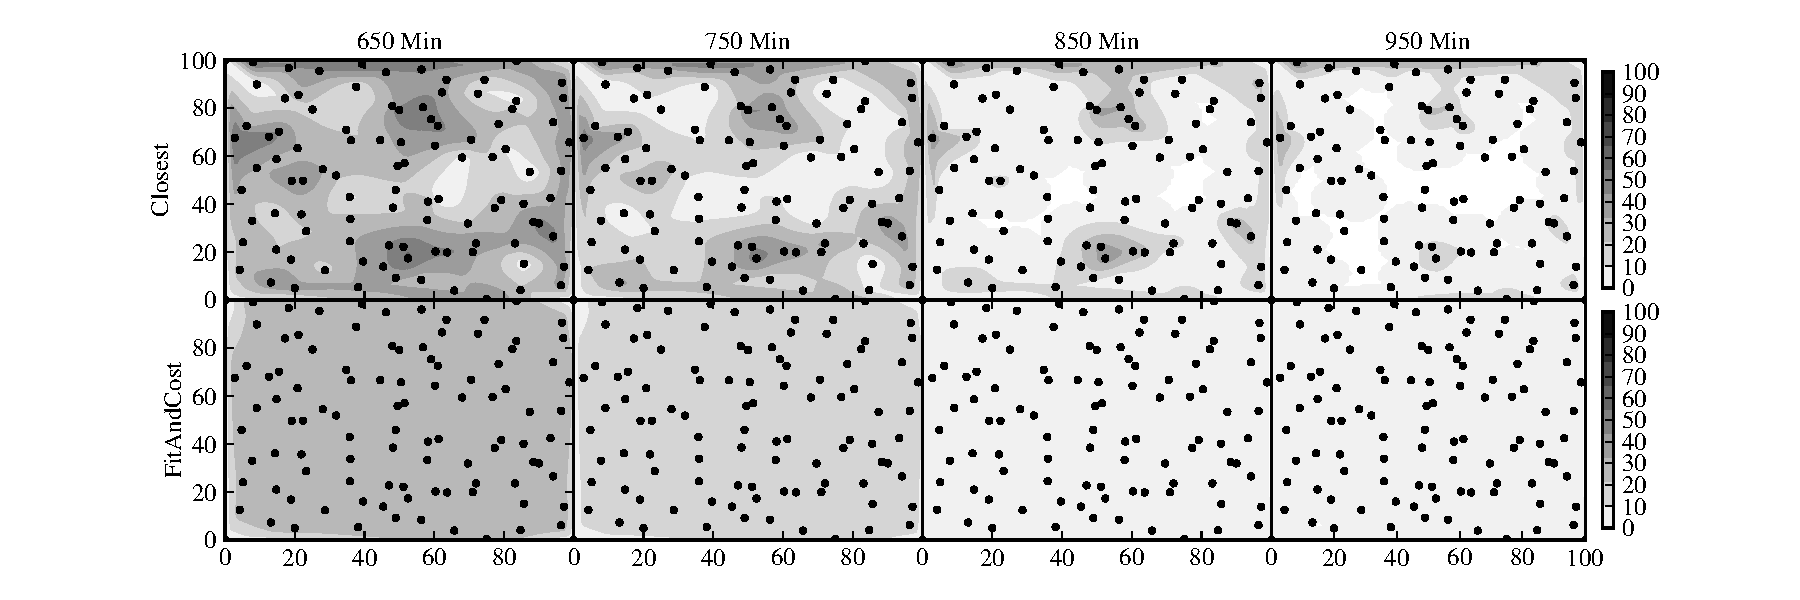
\includegraphics[width=\hsize]{./5-idea/figs/localizationdensityvtime.pdf}
\end{center}

\caption{\textbf{Energy density over time.} Energy densities for the
\texttt{Closest} heuristic and IDEA using the \texttt{WeightedEnergy}
objective function are shown at four points in time. The event distribution
is uniform. IDEA enables better load distribution, which leads to a longer
application lifetime.}

\label{idea-fig-localizationdensityvtime}
\end{figure}

For these experiments we arranged 100 nodes into a 100~m by 100~m area,
resulting in the placements shown in
Figure~\ref{idea-fig-localizationdensityvtime}. We simulate a sensing range
equal to the communication range, each set to 20~m. This radius is chosen to
give each node reasonable number of neighbors and allow it to detect a
reasonable number of events. We randomize the reliable transfer protocol
bandwidth across each link to between 768 and 1280~bytes/sec, a feasible
range based on results from data transfer protocols such as
Flush~\cite{flush-sensys07} and Fetch. Events are simulated using a uniform
random distribution so that events have equal probability of occurring
anywhere in the sensor field.

To evaluate network performance, we define \textit{capability} of the network
as the percent of the last 100 operations that succeeded, where success is
defined as localizing the event. We assume that the application requires that
the network be able to be able to localize a high percentage of events that
occur, and design our energy objective functions with this in mind. As an
example, an intruder localization application is no longer useful once it
fails to detect a very high percentage of intrusion attempts. We quote the
system lifetime as the the 90\% capability time, the time at which the
network's capability drops below 90\%.

We experimented with several approaches to choosing a localization plan, one
that does not use IDEA and three that do using different energy objective
functions:

\begin{enumerate}

\item \textbf{\texttt{Closest}:} produces a localization plan with the node
closest to the event source as the aggregator and the three next closest
nodes as signal providers. We assume a real solution would use an imperfect
estimate of proximity such as total signal energy or signal-to-noise ratio,
but for the simulations we use the known simulated event location to choose
the closest nodes. \texttt{Closest} does not require energy state information
and so could be implemented without IDEA. It is implemented as an example of
a plausible non-energy-aware solution.

\item \textbf{\texttt{MaxEnergy}:} chooses the node with the most energy
(that heard the event) as aggregator and the next three highest-energy nodes
as signal providers.

\item \textbf{\texttt{TotalEnergy}:} chooses the localization plan that
consumes the lowest amount of total energy summed across all nodes in the
network.

\item \textbf{\texttt{WeightedEnergy}:} weights the total energy consumption
using a similarity metric derived from the cosine similarity index to measure
the degree to which the energy vector for the localization plan is a good
``fit'' given the current energy availability.

\end{enumerate}

\begin{figure}[t]
\begin{center}
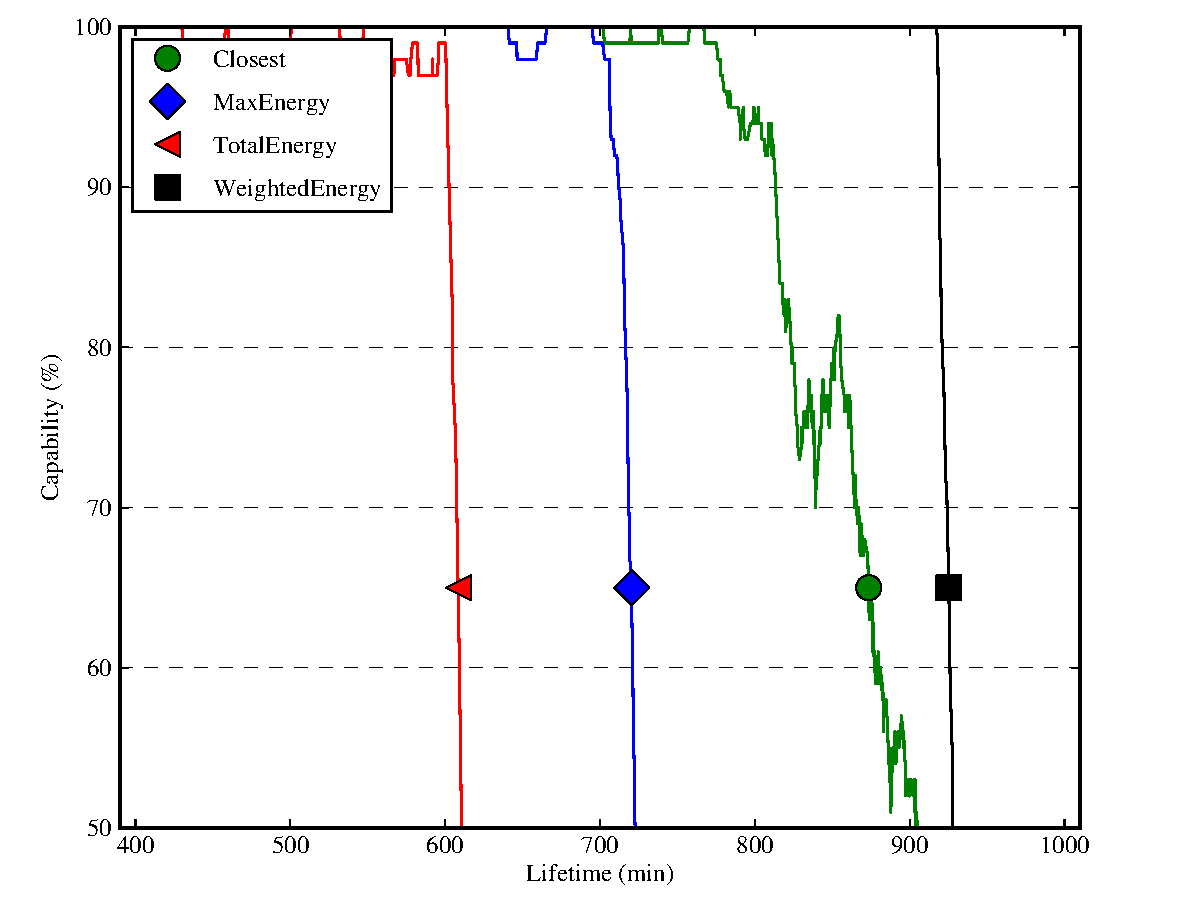
\includegraphics[width=0.7\hsize]{./5-idea/figs/ideavheuristics.pdf}
\end{center}

\caption{\textbf{Performance of IDEA objective functions and heuristic.}
Simulation results are shown for the localization application. The graph
compares the \texttt{Closest} heuristic, implemented without using IDEA,
against three different IDEA objective functions: \texttt{MaxEnergy},
\texttt{TotalEnergy} and \texttt{WeightedEnergy}. The \texttt{WeightedEnergy}
approach using IDEA outperforms the non-energy-aware approach while the other
objective functions perform more poorly.}

\label{idea-fig-ideavheuristics}
\end{figure}

We began by experimenting with the \texttt{Closest}, \texttt{MaxEnergy} and
\texttt{TotalEnergy} approaches. As Figure~\ref{idea-fig-ideavheuristics}
shows, the \texttt{Closest} heuristic outperformed the two IDEA-based
approaches. However, when examining the energy density plot shown in
Figure~\ref{idea-fig-localizationdensityvtime} for the \texttt{Closest}
heuristic we could see that it led to concentrations of available energy on
nodes at dense locations on the irregular grid, while \texttt{MaxEnergy} did
a better job of exhausting all nodes simultaneously, as evidenced by the
extremely sharp drop in network capability it produces. This is despite the
uniform distribution of acoustic event sources, which one might expect to
produce good energy load distribution without the need for tuning.

Our analysis determined that the \texttt{MaxEnergy} suffers because it will
always route data through extra nodes in order to reach the node with the
most energy. So if that node is on the edge of the cluster of nodes that
heard the event, energy may be consumed by nodes within the interior in order
to allow the signal provides to communicate with the aggregator.
\texttt{MaxEnergy} leads to an even usage of energy across the network, but a
short lifetime, because it always prioritizes the distribution of energy over
the amount consumed when choosing how to localize each event.

In contrast, \texttt{Closest}, while it performs better, has the opposite
problem. While it does not consider energy directly, the effect of the
heuristic is to choose based on the total amount of energy consumed. By
selecting the nodes closest to the event, the heuristic almost always leads
to clusters where all signal providers can communicate with the aggregator,
so no extra energy expenditures by other nodes for routing are needed.
However, the non-uniform distribution of nodes means that some nodes more
likely to be the closest node than others, leading to unequal energy
distribution. While the lifetime is better than \texttt{MaxEnergy}, the
existence of energy at some nodes once the capability drops below 90\% led us
to believe that a hybrid approach was possible that would outperform both
\texttt{MaxEnergy} and \texttt{Closest}.

After exploring several additional approaches we found an energy objective
function capable of producing extremely good load distribution, the
\texttt{WeightedEnergy} approach described above.
Figure~\ref{idea-fig-ideavheuristics} shows that it outperforms
\texttt{Closest}, increasing the network's lifetime by 15\%, while
Figure~\ref{idea-fig-localizationdensityvtime} illustrates how it utilizes
all the nodes' available energy, achieving an even distribution similar to
\texttt{MaxEnergy}. It does this by combining aspects of both earlier
approaches. By weighing the total energy consumed it avoids the extremely
high-energy localization plans that the \texttt{MaxEnergy} function will
sometimes use. By also weighing the ``fit'' using the cosine similarity
metric we address unequal energy distribution in a way that the
\texttt{Closest} heuristic does not.

Our experience with the localization application illustrates the role of the
proper energy objective function in enabling good application performance,
and points to the increases in system lifetime possible through better energy
distribution. 
